\documentclass[acmsmall,screen,review,nonacm]{acmart}
\usepackage{mathpartir,stmaryrd,booktabs,array,listings,tikz,xurl,anyfontsize}
\usetikzlibrary{arrows.meta,positioning,fit}
\settopmatter{printacmref=false}
\setcopyright{none}
\citestyle{acmauthoryear}
\definecolor{inkblue}{RGB}{24,67,108}
\definecolor{softblue}{RGB}{240,245,249}
\definecolor{mutedgreen}{RGB}{44,102,77}
\lstdefinelanguage{Klara}{morekeywords={def,defn,fn,let,letfn,if,do,quote,code,esc,run,lift,handle,perform,fork,adopt!,own,read,borrow,freeze,update!,specialize},sensitive=true,morecomment=[l]{;},morestring=[b]"}
\lstset{language=Klara,basicstyle=\small\ttfamily,keywordstyle=\color{inkblue}\bfseries,commentstyle=\color{mutedgreen},stringstyle=\color{mutedgreen},backgroundcolor=\color{softblue},frame=single,rulecolor=\color{softblue},columns=fullflexible,keepspaces=true,showstringspaces=false,breaklines=true,aboveskip=8pt,belowskip=8pt}
\newcommand{\kw}[1]{\mathsf{#1}}
\newcommand{\cfg}[3]{\langle #1;#2;#3\rangle}
\newcommand{\bind}{\mathbin{>\!\!>\!=}}
\newcommand{\step}{\longrightarrow}
\newcommand{\steps}{\longrightarrow^{*}}
\newcommand{\bigj}[3]{#1\vdash #2\Downarrow #3}
\newcommand{\den}[1]{\llbracket #1\rrbracket}
\newcommand{\sub}[3]{#1[#2/#3]}
\newcommand{\app}[2]{\kw{app}(#1,#2)}
\newcommand{\lam}[1]{\kw{lam}(#1)}
\newcommand{\fix}[1]{\kw{fix}(#1)}
\newcommand{\lit}[1]{\kw{lit}(#1)}
\newcommand{\handling}[4]{\kw{handling}(#1,#2,#3,#4)}
\newcommand{\code}[1]{\kw{code}(#1)}
\newcommand{\esc}[1]{\kw{esc}(#1)}
\newcommand{\run}[1]{\kw{run}(#1)}
\newcommand{\WS}{\kw{WS}}
\newcommand{\WSW}{\kw{WSW}}
\newcommand{\WSC}{\kw{WSC}}
\newcommand{\src}[1]{{\normalfont\nolinkurl{#1}}}
\newcommand{\status}[1]{\textsf{\small[#1]}}
\newcolumntype{L}[1]{>{\raggedright\arraybackslash}p{#1}}
\title{Klara: Forkable, Inspectable Computation with Accounted Authority}
\author{Christian Weilbach}
\authorsaddresses{}
\renewcommand{\shortauthors}{C. Weilbach}
\raggedbottom
\begin{document}
\begin{abstract}
A running simulation is more useful when it can be inspected, forked, edited,
and compared with its alternatives. Persistent data makes snapshots cheap,
but does not make file handles, evidence, budgets, or mutable regions safe to
copy. Klara is an experimental Lisp that separates shared computational state
from authority to act. Immutable definition worlds and explicit continuations
support branching; a dynamic authority store controls splitting and settlement;
staging and guarded compilation move selected checks away from repeated use.
We present the language through executable examples, a mechanized small-step
core with lexical effects and staging, a terminating pure big-step account,
and a proposed weighted-tree interpretation of discrete effects. The core has
kernel-checked determinism, progress modulo named failures, and preservation
of de Bruijn well-scopedness. Those results do not yet cover the authority
store or the compiler. Recorded implementation experiments demonstrate certified
pipeline fusion, affine-region lowering, and deoptimization after an effect
without replaying it, while also exposing substantial entry overhead. The
research question is whether one explicit account of authority can support
interactive branching and selective optimization without making their
correctness depend on hidden host state.
\end{abstract}
\keywords{effect handlers, staging, persistent worlds, affine resources, operational semantics, interactive programming}
\maketitle
\noindent\textbf{Internal discussion draft, 28 October 2026.}
Target: OOPSLA 2027, Round 2. This document describes checkout
\src{0831749af6a4} through implementation milestone S11. Results labeled
\emph{checked} refer to repository proofs and recorded runs, not a new
verification run for this draft. Later worktrees are outside this snapshot.

\section{Introduction}
Suppose a simulator is halfway through an experiment when its designer discovers
a better transition rule. Restarting loses the state that made the discovery
interesting. Editing a global definition risks silently changing every running
experiment. Copying the simulator's heap is not enough either: two copies can
spend the same budget, count the same observation twice, or send competing
messages to the outside world.

Klara makes this situation a language-design problem. A \emph{world} is an
immutable root of definitions; a running computation has a basis in that world.
An edit publishes a new root. Forks share the old root and then diverge.
Lexical effect handlers expose continuations as data, so a handler can explore
more than one future. Crucially, the right to perform an action is not conferred
by copying the value that names it. A separate store records who may use a
resource, how its shares divide, and whether it has already been settled.

The following excerpt from guide chapter 4 isolates the distinction. Both
alternatives can refer to \src{e}, but each receives only half its evidence.
Adopting the first commits its expenditure; discarding the second restores its
unused share.
\begin{lstlisting}
(def e (evidence 1))
(fork [a (spend! e 1/4) b (remaining e)]
  (adopt! a)
  (:value b))                    ; => 1/2
(remaining e)                    ; => 3/4
\end{lstlisting}
Evidence accounting is distinct from real expenditure: a budget charges work
performed in discarded branches too. Similarly, a resource explicitly
transferred to one branch stays consumed if that branch is discarded. These
are different meanings of ``fork,'' not different representations of one
unrestricted copying operation.

Our proposed thesis is that \emph{forkable computation needs explicit authority,
and inspectable authority gives optimization a place to justify removing
checks}. The current system supports this thesis in three different ways.
First, it implements a language in which worlds, continuations, code, and
selected authority operations can be inspected and combined. Second, it has a
small executable formal core with proofs that delimit ordinary evaluation and
staging failures. Third, it experiments with moving checks from each dynamic
use to a guarded boundary or a checked local derivation. The last two do not
yet establish a theorem about the whole first system.

The draft's contributions are:
\begin{enumerate}
\item A language-design account of the interaction between immutable worlds,
lexical effects, authority-sensitive branching, staging, and affine regions
(Sections~\ref{sec:overview} and~\ref{sec:authority}). The combination and its
failure boundaries are the intended contribution; the ingredients have substantial
prior art.
\item A faithful presentation of the mechanized operational core, including
its locally nameless staging machinery and exact proof scope
(Section~\ref{sec:core}); a new, unmechanized big-step equivalence sketch for a
pure fragment (Section~\ref{sec:big}); and a deliberately restricted denotational
proposal with an explicit adequacy obligation (Section~\ref{sec:den}).
\item An implementation account connecting proof-checked fusion and checked
affine derivations to guarded compilation and exact frame reconstruction, with
recorded positive and negative measurements (Sections~\ref{sec:impl}
and~\ref{sec:eval}).
\end{enumerate}
A submission should sharpen the first contribution into an authority theorem
and strengthen the third with independent repeated measurements. This draft
keeps those gaps visible so it can serve as a discussion artifact, rather than
presenting a completed verification story.

\section{A Language for Exploring Alternatives}\label{sec:overview}
\subsection{Definitions belong to worlds}
Klara uses a Clojure-like surface over a small core. Expansion records the
world facts it reads, including macro identities, inspected values, and absent
names. Ordinary references retain late lookup; merely mentioning a non-macro
definition does not inline its value. Definitions are published by compare-and-swap
on a root containing definitions and dependency information. An unchanged
canonical expanded term retains its CodeId, permitting early cutoff.

The guide's price example makes world isolation observable:
\begin{lstlisting}
(defn price [x] (* x 10))
(def w (perform :world/fork))
(perform :world/eval-in w '(defn price [x] (* x 12)))
[(price 3) (perform :world/eval-in w '(price 3))]
; => [30 36]
(defn price [x] (* x 11))
[(price 3) (perform :world/eval-in w '(price 3))]
; => [33 36]
\end{lstlisting}
Snapshot creation shares the persistent root; it does not copy every definition.
A stored open closure is resolved under the caller's basis. A closure created
while executing instead pins its creation basis. Consequently, raising a
fiber's basis does not retroactively change all its existing closures. The
running-simulation example explicitly resolves its transition at each step:
its recorded states are $0,1,2$, then $12,22$ after a basis raise changes the
increment from $1$ to $10$ (\src{examples/klara/09-basis-raise.md}). This is an
opt-in update point, not arbitrary replacement of live JVM frames.

Publication and repair are distinct. Broken expansion reads can leave a
definition pending until invalidation re-expands it; the REPL performs this
repair automatically. A future persistence story must preserve this distinction
and record host dependencies that expansion currently cannot see.

\subsection{Lexical effects expose control}
A handler binds an instance; a perform explicitly names that instance. Equal
operation names in unrelated handlers do not by themselves cause interception.
The handler supplies the operation's arguments and a deep resumption:
\begin{lstlisting}
(handle [h {:split (fn [k] [(k :left) (k :right)])}]
  (let [x (perform h :split)]
    {:branch x :n (count (str x))}))
; => [{:n 5, :branch :left} {:n 6, :branch :right}]
\end{lstlisting}
The clause runs outside the handler; invoking its continuation reinstalls the
handler. Ambient operations instead use an explicit dynamic mode. World,
host, time, and stage operations have reference interpretations. The authority
and ownership operations are protected runtime boundaries, not user-replaceable
ambient handlers. T0 can capture its own data frames, but cannot capture a
continuation across an opaque host callback frame.

This control interface is sufficient to express an instructional particle
filter (\src{examples/klara/07-smc.md}). At an observation, particles suspend;
resampling selects continuations to resume. The recorded two-state hidden
Markov model has exact final posterior $279711/316123\simeq0.884817$ and
normalizer $0.030347808$. A 1,000-particle run at seed 42 reports $0.896$ and
$0.0300642860$. This illustrates the interface, not an inference-correctness
proof: the example manages weights and keys as ordinary values, and its separate
authority demonstration does not certify the entire SMC algorithm.

\subsection{Adoption makes effects observable}
The \src{fork} form evaluates alternatives sequentially in the prototype,
then runs a body that may adopt at most one. Classified irreversible host
calls become intents inside these explicit branches:
\begin{lstlisting}
(fork [a (println "send offer A")
       b (println "send offer B")]
  (adopt! b) :sent)
; prints: send offer B
; => :sent
\end{lstlisting}
An explicitly transferred capability can authorize an immediate action instead;
a receipt records it. This is not a transactional wrapper around arbitrary
Java code. Classification covers known or annotated host calls at the
\src{:host/call} boundary; unclassified host mutation remains outside the model.
Nor do repeated handler resumptions automatically inherit the intent mechanism.

\begin{figure}[t]
\centering
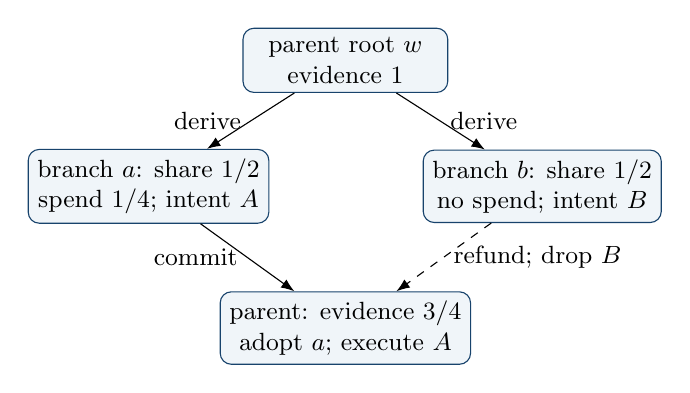
\begin{tikzpicture}[>=Latex,font=\small,box/.style={draw=inkblue,rounded corners,fill=softblue,align=center,minimum width=2.6cm,minimum height=.8cm}]
\node[box] (p) at (0,0) {parent root $w$\\evidence $1$};
\node[box] (a) at (-2.5,-1.6) {branch $a$: share $1/2$\\spend $1/4$; intent $A$};
\node[box] (b) at (2.5,-1.6) {branch $b$: share $1/2$\\no spend; intent $B$};
\node[box] (q) at (0,-3.4) {parent: evidence $3/4$\\adopt $a$; execute $A$};
\draw[->] (p)--node[left]{derive}(a); \draw[->] (p)--node[right]{derive}(b);
\draw[->] (a)--node[left]{commit}(q); \draw[->,dashed] (b)--node[right]{refund; drop $B$}(q);
\end{tikzpicture}
\caption{Schematic composition of the guide's evidence and intent examples.
Data roots share structure; authority is derived and settled. Discard refunds
evidence, but would still charge budget expenditure. The diagram is not an
additional executed transcript.}\label{fig:fork}
\Description{A parent derives two half-shares of evidence; branch a spends one quarter and is adopted, while branch b is discarded and refunded.}
\end{figure}

A coupled fork deliberately gives alternatives common random numbers. In the
recorded city example, 40 paired runs yield a difference estimate with sample
standard deviation 152, versus 353 for independent runs; the corresponding
means are 2940 and 2906, against an expected difference of 2925. These small
experiments motivate the API. They establish neither statistical independence
of split streams nor a general variance-reduction theorem.

\subsection{Code is an inspectable value}
Staging distinguishes a term's execution from its construction. \src{code}
raises the stage and \src{esc} evaluates at the surrounding stage, splicing a
code value. Here is the guide's power generator, with transcript output shown
as comments and the final application parenthesized conventionally:
\begin{lstlisting}
(def power
  (fn [n x]
    (if (zero? n) (code 1)
      (code (* (esc x) (esc (power (dec n) x)))))))
(code (fn [y] (esc (power 3 (code y)))))
; => (code (fn [y_1] (* y_1 (* y_1 (* y_1 1)))))
((run (code (fn [y] (esc (power 3 (code y)))))) 2)
; => 8
\end{lstlisting}
Generated binders receive fresh names, and runtime scope checks reject a splice
whose free generated names have escaped their binding extent. \src{run} checks
closedness and evaluates under the current basis, using T0 in this snapshot.
It is not yet a general staged-code-to-host compiler.
A mutable host cell can carry open code beyond the construction of its binder;
the following recorded guide example is rejected at the later splice:
\begin{lstlisting}
(let [r (atom nil)]
  (code (fn [x] (esc (do (reset! r (code x)) (code x)))))
  (code (fn [y] (esc @r))))
; scope-extrusion: x's binder is no longer in scope
\end{lstlisting}
The error comment abbreviates the transcript diagnostic. Naming the second
binder \src{x} instead would not repair the escaped binding's identity.

\src{genlet} shares residual computations by inserting a binding as far out as
its free variables allow. Floating above a conditional or lambda may make a
computation run earlier or more often. Purity alone is insufficient: failure
and divergence must also be preserved. The generator's author currently bears
this obligation. Memoized recursive let-insertion supports a variable-size
recursive group; neither insertion operation is in the formal core.

\subsection{Optimization has an observable fallback}
Guide chapter 6's certified pipeline sums squares of selected numbers. With an
even predicate, the input $[1,2,3,4,5,6]$ gives $56$; redefining the predicate to
odd gives $35$ through the generic path until reoptimization. A proof about a
list fold licenses fusion, while world and host-handler guards determine
whether that proof's interpretation is applicable at this call.

Guide chapters 8--9 extend the story to guarded compilation and affine regions.
In the recorded \src{paid-add} example, evidence is spent before a numeric
speculation. Calling compiled code with $1.5$ returns $[4.0,3/4]$: a failed
Long guard resumes T0 after the expenditure, without spending again. Local
owned cells can be updated, borrowed for reading, and frozen to persistent
values. A recorded example returns old snapshots $[1,2]$ alongside a final
$[1,2,3,4]$:
\begin{lstlisting}
(let [before [1 2] o (own before) snapshot (read o)]
  (update! o conj 3 4)
  [before snapshot (freeze o)])
; => [[1 2] [1 2] [1 2 3 4]]
\end{lstlisting}
No snapshot is silently mutated. These behaviors are tested implementation
properties; the next sections say exactly what is proved.

\section{The Mechanized Core}\label{sec:core}
The executable specification lives in \src{spec/src/klara/spec/}.
\src{core.clj} defines syntax and a total one-step evaluator; \src{ws.clj}
defines scoping and its supporting lemmas; \src{props.clj} contains the
metatheorems; \src{interp.clj} bridges terms to an executable host interpreter.
Ansatz implements a Lean-4-style dependent type theory and kernel on the JVM,
with Clojure proof syntax. ``Kernel-checked'' below means checked there; an
independent recheck by upstream Lean 4 is not part of the recorded artifact.

\subsection{Syntax, binding, and configurations}
The twelve source forms are below. Indices $i$, world identifiers $a$, and
operation tags $o$ are naturals; $d$ is nil, a boolean, or a mathematical integer.
\[
\begin{array}{rcl}
t &::=& \kw{var}(i)\mid\lit d\mid\lam t\mid\app t t
       \mid\kw{let}(t,t)\mid\kw{if}(t,t,t)\\
 &&{}\mid\kw{letrec}(t,t)\mid\kw{resolve}(a)\mid\kw{prim}(p,t,t)\\
 &&{}\mid\kw{perform}(o,t,t)\mid\kw{handle}(t,t,t)
       \mid\kw{specialize}(t,t),\\
p &::=& +\mid -\mid *\mid =\mid <.
\end{array}
\]
Staging adds $\code t$, $\esc t$, and the spec-only spelling $\run t$.
T0 expresses the last via the ambient \src{:stage/run} operation. Runtime
constructors are $\fix b$, $\kw{cap}(\ell)$, $\handling\ell b r q$,
$\kw{gvar}(g)$, and named forms $\kw{nlam}$, $\kw{nlet}$,
$\kw{nletrec}$, $\kw{nhandle}$. Together these are the spec's 23 constructors;
not every constructor is a surface expression.

A lambda binds index 0. A recursive function body binds argument 0 and self 1;
its surrounding letrec body binds self 0. A handler's body binds its capability
at 0, its return clause binds the result at 0, and its operation clause binds
continuation 0, argument 1, and integer operation tag 2. The spec has one
operation-dispatch clause and unary functions; T0 adds maps of named clauses,
multiple arguments, rest arguments, mutual recursion, and richer host data.

Write $\sub t v i$ for the spec's index-lowering substitution: it replaces $i$
and lowers larger free indices by one, respecting binder depths. In ordinary
execution the substituted values are de Bruijn closed, so no shifting of their
free indices is needed. Staging opens binders with generated names instead of
reducing under de Bruijn binders.

A configuration is $\cfg w n t$, with an association-list world $w$ and a fresh
name/label counter $n$. The ordinary syntactic values are
\[
 v ::= \lit d\mid\lam b\mid\fix b\mid\kw{cap}(\ell).
\]
This is precisely \src{isVal}, not the complete staged value predicate. The
staged evaluator recognizes built code values through its \src{Out.val}
outcome. Its scoping predicate $\WS_k(t)$ checks de Bruijn indices; generated
names are permitted without a freshness premise. $\WSW(w)$ requires stored
terms to be closed, and $\WSC(\cfg w n t)$ combines world and term scoping.
It does \emph{not} require world entries to be values, prove freshness of $n$,
or establish capability uniqueness.

\subsection{Small-step evaluation}
Let $\cfg w n t\step\cfg w {n'}{t'}$ mean that the spec's optional step returns
$(n',t')$. Figures~\ref{fig:pure} and~\ref{fig:effects} present the level-zero
rules on the ordinary fragment. They are a relational presentation of a
functional definition, not a separately mechanized rule set.
\begin{figure}[p]
\begin{mathpar}
\inferrule*[right=Beta]{v\text{ value}}{\cfg w n {\app{\lam b}v}\step\cfg w n {\sub b v0}}
\and
\inferrule*[right=RecBeta]{v\text{ value}}{\cfg w n {\app{\fix b}v}\step\cfg w n {b[\fix b/1][v/0]}}
\and
\inferrule*[right=Let]{v\text{ value}}{\cfg w n {\kw{let}(v,b)}\step\cfg w n {b[v/0]}}
\and
\inferrule*[right=Letrec]{ }{\cfg w n {\kw{letrec}(f,b)}\step\cfg w n {b[\fix f/0]}}
\and
\inferrule*[right=If]{\kw{truth}(v)=j}{\cfg w n {\kw{if}(v,b_1,b_0)}\step\cfg w n {b_j}}
\and
\inferrule*[right=Resolve]{\kw{lookup}(w,a)=t}{\cfg w n {\kw{resolve}(a)}\step\cfg w n t}
\and
\inferrule*[right=Prim]{\delta_p(d_1,d_2)=d}{\cfg w n {\kw{prim}(p,\lit{d_1},\lit{d_2})}\step\cfg w n {\lit d}}
\and
\inferrule*[right=Specialize]{p,m\text{ values}}{\cfg w n {\kw{specialize}(p,m)}\step\cfg w n {\lam{\app{\app p m}{\kw{var}(0)}}}}
\and
\inferrule*[right=Context]{\cfg w n t\step\cfg w {n'}{t'}}{\cfg w n {E[t]}\step\cfg w {n'}{E[t']}}
\end{mathpar}
\caption{Ordinary reductions. Evaluation contexts are left-to-right CBV:
function then argument; initializer of let; condition of if; both primitive
operands; target then argument of perform; both specialization operands; and
body of an installed handler. No ordinary context crosses a de Bruijn binder.
Truth is false exactly for nil and false. $\delta$ is partial on datum types;
missing definitions and invalid applications give named failures.}\label{fig:pure}
\Description{Inference rules for ordinary call-by-value reduction, including recursion, lookup, primitives and partial application.}
\end{figure}

\begin{figure}[t]
\small
\begin{mathpar}
\inferrule*[right=Handle]{ }{\cfg w n {\kw{handle}(b,r,q)}\step
 \cfg w {n+1}{\handling n {b[\kw{cap}(n)/0]}r q}}
\and
\inferrule*[right=Return]{v\text{ value}}{\cfg w n {\handling\ell v r q}\step\cfg w n {r[v/0]}}
\and
\inferrule*[right=Operation]{E\text{ contains no handler for }\ell\\
 k=\lam{\handling\ell {E[\kw{var}(0)]}r q}}
 {\cfg w n {\handling\ell {E[\kw{perform}(o,\kw{cap}(\ell),v)]}r q}
 \step\cfg w n {q[k/0][v/0][\lit{\kw{int}(o)}/0]}}
\end{mathpar}
\caption{Lexically targeted deep handlers. Each substitution in the operation
rule uses index 0 because the previous substitution removes a binder. The
clause executes outside this handler; the resumption installs it again.}
\label{fig:effects}
\Description{Rules for handler allocation, return, and lexically targeted operation handling with a deep resumption.}
\end{figure}

The operation rule deserves care: writing successive substitutions at indices
$0,1,2$ would be incorrect for this substitution function. The operation tag
must also be injected into a literal integer. A handler with a different
label is part of the captured context and forwards the operation. A nil target
is ambient and remains unhandled by this core; any other target that is not
a capability yields \src{badTarget}. The deterministic evaluator is not a
random evaluator: probabilistic branching is an interpretation chosen by a
handler that may invoke its continuation repeatedly.

\subsection{Staging as level-indexed construction}\label{sec:stages}
The implementation of one step is $\kw{ev}(w,n,t)(s)$, structurally recursive
on $t$ and then applied to stage $s$. Its outcomes are
\[
\kw{val},\quad\kw{next}(n',t'),\quad\kw{eff}(h,o,v,E),\quad
\kw{stuck}(a),\quad\kw{chk}(G,n',t').
\]
An effect outcome accumulates a context while bubbling; a check outcome
accumulates the generated names that must still be in scope. At a positive
level, applications, conditionals, primitives, and effects are constructed
rather than executed. In particular both branches of a residual conditional
are built, so their escapes can run during generation.

For clarity, write $t\rightsquigarrow_s^{n,n'}t'$ for an \src{Out.next}
outcome of this evaluator. Representative constructor rules are:
\begin{mathpar}
\inferrule*[right=OpenLam]{s>0}{\lam b\rightsquigarrow_s^{n,n+1}
  \kw{nlam}(n,b[\kw{gvar}(n)/0])}
\and
\inferrule*[right=QuoteStep]{b\rightsquigarrow_{s+1}^{n,n'}b'}
 {\code b\rightsquigarrow_s^{n,n'}\code{b'}}
\and
\inferrule*[right=EscBuild]{s>1\quad b\rightsquigarrow_{s-1}^{n,n'}b'}
 {\esc b\rightsquigarrow_s^{n,n'}\esc{b'}}
\and
\inferrule*[right=Run]{\kw{ev}(w,n,\code c)(0)=\kw{val}\\
 u=\kw{toDB}(c)\quad\kw{wsbF}(u,0)=\kw{true}}
 {\run{\code c}\rightsquigarrow_0^{n,n}u}
\end{mathpar}
The quote and escape contexts also propagate effects, stuck outcomes, and
checks; the rules above intentionally show only their stepping case. Once
\src{esc} at level 1 has evaluated its argument at level 0 to built
$\code c$, it returns $\kw{chk}(\kw{fnames}(c),n,c)$, not an unconditional
splice step. Each enclosing named binder discharges the names it binds from
this list. An empty list becomes a step; names left at the boundary yield
\src{scopeExtrusion}. Running code whose de Bruijn conversion is not closed
also yields \src{scopeExtrusion}. Escape at level 0 is a stage error.

Named let opens one name; named letrec opens the argument $n$ and self $n+1$.
Named handle opens five: capability $n$, return variable $n+1$, continuation
$n+2$, argument $n+3$, operation $n+4$. The staged handler builds its operation
clause, then return clause, then body, as in \src{ev}; ordinary CBV order
alone does not specify this order. A generated variable at level 0 evaluates
to its own code; at positive levels it is already built syntax. A recursive
\src{fix} value is opaque at every level. Capabilities and installed handlers
cannot be lifted to positive levels.

This locally nameless machinery keeps de Bruijn substitution simple, but
well-scopedness is intentionally weaker than a theorem that generated names
never collide or escape. A named extrusion failure is an allowed result of a
well-scoped computation. T0 additionally checks liveness of generated binding
scopes and implements \src{lift}; the spec's cross-stage persistence is
substitution. Section~\ref{sec:diff} records observable differences.

\subsection{What the proofs establish}\label{sec:proofs}
\begin{theorem}[Determinism, kernel-checked]
If $c\step c_1$ and $c\step c_2$, then $c_1=c_2$.
\end{theorem}
The theorem \src{step-det} follows because the relation is the graph of a
function. This proves uniqueness of the specified next step, not agreement
with the larger T0 runtime.
\begin{theorem}[Progress modulo named outcomes, kernel-checked]
For a configuration satisfying $\WSC$, evaluation either recognizes a value,
steps, exposes an unhandled effect, or reaches a named failure other than the
unbound de Bruijn variable failure \src{scope}. An outstanding scope check may
be reported as scope extrusion.
\end{theorem}
\begin{theorem}[Preservation, kernel-checked]
If $\WSC(c)$ and $c\step c'$, then $\WSC(c')$.
\end{theorem}
The common lemma \src{ev-ok} reasons about all levels of the evaluator.
\src{progress-config}, \src{preservation-config}, and the multi-step safety
corollary use it. This is preservation of \emph{scoping}, not a typed
``programs cannot go wrong'' theorem: bad applications, primitive type errors,
missing definitions, stage errors, and unhandled effects remain expressible.

For closed syntactic values $p,m,x$, \src{smn} proves that
$\app{\kw{specialize}(p,m)}x$ takes exactly two steps to $\app{\app p m}x$.
Determinism then gives the associated terminal-result equivalence. Evaluating
an effectful expression for $m$ twice is not covered; neither are all staged
values, which are not characterized by \src{isVal}. The checked \src{run-quote}
lemma covers only the binder-free \src{Quotable} fragment, not arbitrary code
with lambdas, nested brackets, or escapes.

\begin{table}[t]
\caption{Claim ledger. Checked means the repository reports ansatz kernel checking;
we did not rerun a JVM. ``Tested'' never means a universal theorem.}
\label{tab:status}
\small
\begin{tabular}{L{.32\linewidth}L{.21\linewidth}L{.37\linewidth}}
\toprule Claim & Status & Exact boundary\\\midrule
Determinism; progress; scoping preservation & Checked & Small-step spec including staging; named failures allowed\\
Value s-m-n; run/quote & Checked & Simple values; binder-free Quotable respectively\\
Fold/map and fold/filter laws & Checked & Kernel list model and per-pipeline equation\\
Big-step/small-step equivalence & Proof sketch here & Closed, pure, unstaged fragment\\
Finite-tree bind/fold law & Elementary proof here & Finite discrete trees only\\
Probabilistic operational adequacy & Conjecture & Needs reference-handler and numeric relation\\
Authority conservation; no stale use & Implemented and tested & S6/S10; absent from core proofs\\
Affine check erasure & Checked derivations; tested lowering & No kernel soundness theorem\\
Deoptimization trace preservation & Implemented and tested & Supported frame states; no simulation proof\\
Full T0 refinement; full denotation & Open & Host, worlds, authority, general recursion, staging\\
\bottomrule
\end{tabular}
\end{table}

\section{A Big-Step Account of the Pure Fragment}\label{sec:big}
This section is a new paper-level definition and proof sketch, not a claim
about existing ansatz declarations. Let $\mathcal P$ be the sublanguage with
variables, literals, lambda, application, let, if, letrec, resolve, primitives,
and specialize. Exclude handlers, perform, capabilities, and all staging and
named constructors; allow runtime fix values. Fix a world whose reachable
entries are closed $\mathcal P$ terms. They need not terminate, and need not
be values. We define only successful terminating evaluation, using substitution
rather than environments so that the relation to the spec is direct.

The judgment $\bigj w t v$ means that $t$ evaluates to a pure value $v$
(literal, lambda, or fix). Let $B(\lam b,u)=b[u/0]$ and
$B(\fix b,u)=b[\fix b/1][u/0]$. Undefined $B$ or $\delta$ gives no derivation.
\begin{mathpar}
\inferrule*[right=B-Val]{v\text{ pure value}}{\bigj w v v}
\and
\inferrule*[right=B-App]{\bigj w f v_f\quad\bigj w a u\\
 B(v_f,u)=b\quad\bigj w b v}{\bigj w {\app f a}v}
\and
\inferrule*[right=B-Let]{\bigj w e u\quad\bigj w {b[u/0]}v}
 {\bigj w {\kw{let}(e,b)}v}
\and
\inferrule*[right=B-If]{\bigj w c u\quad\kw{truth}(u)=j\quad\bigj w {b_j}v}
 {\bigj w {\kw{if}(c,b_1,b_0)}v}
\and
\inferrule*[right=B-Rec]{\bigj w {b[\fix f/0]}v}
 {\bigj w {\kw{letrec}(f,b)}v}
\and
\inferrule*[right=B-Resolve]{\kw{lookup}(w,a)=t\quad\bigj w t v}
 {\bigj w {\kw{resolve}(a)}v}
\and
\inferrule*[right=B-Prim]{\bigj w {t_1}{\lit{d_1}}\quad
 \bigj w {t_2}{\lit{d_2}}\quad\delta_p(d_1,d_2)=d}
 {\bigj w {\kw{prim}(p,t_1,t_2)}{\lit d}}
\and
\inferrule*[right=B-Spec]{\bigj w p {v_p}\quad\bigj w m {v_m}}
 {\bigj w {\kw{specialize}(p,m)}{\lam{\app{\app{v_p}{v_m}}{\kw{var}(0)}}}}
\end{mathpar}

\begin{proposition}[Equivalence; unmechanized proof sketch]\label{prop:big}
For closed $t\in\mathcal P$, a world as above, and any $n$,
\[
 \bigj w t v\quad\Longleftrightarrow\quad
 \cfg w n t\steps\cfg w n v\quad(v\text{ a pure value}).
\]
\end{proposition}
\begin{proof}[Proof sketch]
For the forward direction, induct on the big-step derivation. In B-App,
lift the function's reduction through the function context, lift the
argument's reduction through the argument context with the function value
fixed, take Beta or RecBeta, and append the body's reduction. B-Let and
B-If similarly concatenate only the selected computation. B-Resolve takes
one lookup step followed by its premise's reduction, so a world entry is
not silently assumed to be a value. B-Rec and B-Spec take their respective
head steps; B-Prim uses the same partial datum operation.

For the reverse direction establish backward closure:
if $t\step t'$ in $\mathcal P$ and $\bigj w {t'}v$, then $\bigj w t v$.
For head redexes this is the corresponding big-step rule; for contexts,
invert the big-step derivation to obtain the judgment on the subterm,
apply backward closure there by induction on the context, and rebuild the
outer derivation. Pure substitutions preserve this fragment and closedness.
Induct backwards over the finite reduction sequence, starting with B-Val.
No rule in $\mathcal P$ allocates labels or names, so $n$ is unchanged.
\end{proof}
This statement is about successful termination. Absence of a big-step
derivation conflates divergence and named failure; it is not an adequacy
claim for exceptions, effects, or a cost semantics. Extending it to staged
code would require level-indexed values and the explicit check outcomes.

\section{Weighted Trees and Handler Meaning}\label{sec:den}
Research note A and \src{doc/semantics.md} propose a weighted-execution-tree
model. They do not provide a full denotational semantics or an adequacy proof
for Klara. We make a restricted part precise here, to give the proposal a
concrete object of discussion.

\subsection{A finite algebra, not yet a model of all terms}
Fix a first-order operation signature with a set $A_o$ of arguments and a
\emph{finite} set $R_o$ of results for each operation, and a fixed set of
handler labels. For a set $X$ of results, define finite trees
\[
 T X ::= \kw{Ret}(x)\mid\kw{Fail}
       \mid\kw{Op}(\ell,o,a,k),\qquad k:R_o\to T X.
\]
The finite restriction excludes recursion with infinite unfolding and
continuous sampling. Labels here are parameters; modeling their fresh
allocation and escape needs an additional nominal or world-indexed
construction. Higher-order closures are not modeled by simply asserting that
$X$ solves an unrestricted function-space equation.

Define $\kw{Ret}(x)\bind f=f(x)$, $\kw{Fail}\bind f=\kw{Fail}$, and
\[
 \kw{Op}(\ell,o,a,k)\bind f
 =\kw{Op}(\ell,o,a,\lambda r.\,k(r)\bind f).
\]
Here $\bind$ denotes tree substitution at return leaves. A handler with return
interpretation $\eta:X\to Y$ and operations
$H_{\ell,o}:A_o\times(R_o\to Y)\to Y$ with a distinguished failure element $0_Y$ gives a fold:
\[
\begin{split}
\den{\kw{Ret}(x)}_H&=\eta(x),\qquad
\den{\kw{Fail}}_H=0_Y,\\
\den{\kw{Op}(\ell,o,a,k)}_H&=
 H_{\ell,o}(a,\lambda r.\den{k(r)}_H).
\end{split}
\]
This equation captures deep interpretation of the continuation. For a handler
that forwards an operation, $Y$ may itself be a residual-tree carrier; the
clause is interpreted outside the handler while the recursive continuation
uses its fold. It is not a proof that the syntactic substitution rule in
Figure~\ref{fig:effects} has this meaning for higher-order Klara.

\subsection{Discrete scoring and normalization}
For a distinguished label, choose Boolean sampling with parameter
$p\in[0,1]\cap\mathbb Q$ and scoring with $r\in\mathbb Q_{\geq0}$ and unit
result. Let $Y=\mathcal M_f(X)$ be finite-support, finite nonnegative measures.
Use Dirac return, zero failure, and
\[
\begin{split}
 H_{\kw{choose}}(p,k)&=p\,k(\kw{true})+(1-p)\,k(\kw{false}),\\
 H_{\kw{score}}(r,k)&=r\,k(\star).
\end{split}
\]
Thus $\den T_H(x)$ is the sum of products of edge probabilities and scores
along successful paths to $x$. Scores larger than 1 are allowed, so these
are \emph{not necessarily subprobability measures}. For
$Z=\sum_x\den T_H(x)>0$, normalization is
$\kw{norm}(T)=(Z,\den T_H/Z)$. Zero mass is a separate outcome. Extending to
infinite trees or continuous distributions adds measurability, convergence,
and potentially infinite-mass cases. The semantics of scoring and
normalization in higher-order probabilistic languages supplies the relevant
benchmark, not a result inherited automatically by Klara~\cite{staton2016}.

\begin{proposition}[Finite-tree composition; elementary proof]
For the discrete reference interpretation and finite trees,
\[
 \den{T\bind f}_H(y)=\sum_x\den T_H(x)\,\den{f(x)}_H(y).
\]
\end{proposition}
\begin{proof}
Induct on $T$. Return selects the single summand $x$; failure has all
coefficients zero. At choose, distribute the finite sum over the two
weighted branches and apply the induction hypotheses. At score, pull its
nonnegative scalar through the finite sum and apply the hypothesis to its
single child. These exhaust the distinguished signature.
\end{proof}
This small algebraic fact is proved here, but not kernel-checked. Normalization
is nonlinear: normalizing each branch before combining can discard the
relative masses. Evidence accounting must therefore say which mass is shared,
which is newly observed, and what a join is authorized to count.

\subsection{The adequacy obligation}
\textbf{Conjecture (restricted operational adequacy).} For a closed, first-order
program with a finite execution tree, a fixed closed world, no host, authority,
or staging operations, and the discrete choose/score reference handlers,
the unnormalized result measure obtained by operational enumeration equals
$\den{\mathcal T(t)}_H$, where $\mathcal T$ is a compositional elaboration into
the tree algebra preserving call-by-value sequencing and lexical targets.
The elaboration and the simulation relating it to captured contexts remain to
be supplied. The exact rational model also needs an explicit relation to the
prototype's numeric operations; finite test agreement does not replace it.

A full model must account for divergence, higher-order recursive functions,
capability allocation, world updates, and the intensional inspection of code.
The proposed monoidal-computer reading in note A additionally needs a careful
separation between copyable data and linear authority. The checked value
s-m-n law is useful evidence for this direction, but does not construct a
universal evaluator, a retraction for every host type, or a compiler-correctness
theorem. The categorical program remains design work.

\section{Authority and Moving Checks}\label{sec:authority}
\subsection{A store behind aliasable tokens}
RFCs 0001 and 0005 describe authority as an explicit resource discipline.
Operationally, T0 maintains a store
\[
 \Sigma:\kw{Id}\rightharpoonup
 (\kw{kind},\kw{generation},\kw{status},\kw{context},\kw{payload}).
\]
An authority value names an entry; aliases may occur in collections, closures,
metadata, and world definitions. Operations resolve the authority through the
current branch context and check generation and lifecycle at use. Lazy branch
derivation avoids relying on a shallow traversal that could miss an alias.
Copying a token is therefore not minting a second permission.

The lifecycle is open $\to$ advancing $\to$ settled or incomplete. A failed
read-only settlement preflight reopens the authority; a failure after a durable
write marks it incomplete. Repeating a completed identical merge or discard
is idempotent; incompatible settlement is refused. The prototype does not yet
implement recovery from incomplete settlement. An abandoned continuation can
also leave an advancing lease, so fail-closed behavior is not a liveness theorem.
The multi-step protocol assumes a single T0 machine; it is not a proved
concurrent atomic transaction across systems.

\subsection{Resource algebras are a specification direction}
A useful starting point is a partial commutative monoid of compatible shares
$(A,\mathbin\cdot,\epsilon)$ with validity. Exclusive resources compose only
with the unit; evidence shares add; branch ownership composes by disjoint
union of system sets. This connects the design to resource algebras in
separation logic~\cite{iris2018}, but RFC 0005's table is not itself a complete
Iris algebra or proof. Random-key splitting, in particular, has no specified
commutative recombination operation. Budgets with tradable components can
become negative, so a carrier of only nonnegative vectors does not describe
all implemented states. Histories, provenance, lifecycle, and an authoritative
store element are needed in addition to fractions.

The intended conservation obligations can nevertheless be stated. If an
evidence authority of mass $q$ derives shares $q_i$, require
$\sum_iq_i=q$. If branch $j$ is adopted after spending $s_j$, and discarded
branches' evidence is refunded, the parent retains $q-s_j$ (ignoring separately
tracked mints). For a real-cost budget, it retains $q-\sum_i s_i$ instead.
Joining evidence with shared provenance must count a common observation once;
numeric addition alone cannot discover whether observations are independent.
These are requirements for a future transition system over $\Sigma$, not
corollaries of the pure core's progress theorem.

\subsection{Affine islands}
Owned cells extend this store with a payload, a share, a permission mode, and
outstanding loans. Fractional read permissions follow the familiar idea that
shared reads are compatible while writes require full ownership~\cite{boyland2003}.
Klara must also distinguish \emph{mode} from fraction: a read loan of fraction
1 still cannot write. Write access requires full share, write mode, and no
outstanding loans. Scoped cleanup returns the exact borrowed share and
invalidates the loan; freezing consumes the owned handle and returns persistent
data.

A full write authority blocks a fork before alternatives execute. General
continuation capture through an owned region is also rejected; structurally
recognized tail-resumptive or abortive clauses can avoid capture. This creates
an ``affine island'': acquire local ownership, perform updates, freeze, then
fork persistent results. T0 invokes an update function once under an exclusive
lease; failure restores the cell value, but does not undo arbitrary mutation
that a host callback might have performed elsewhere.

The S10 checker recomputes a local derivation for a restricted fragment of
allocations, updates, loans, branching, loops, and settlement. The compiler can
then lower owned cells to private boxes, and a narrower fixed-index literal
Long-vector increment loop to a private array. Snapshots copy the array.
Escaping owned parameters and arbitrary host effects are outside this erasure
fragment. Dynamic boundary checks remain where the local derivation supplies
no ownership fact.

\subsection{Binding time is a proof obligation}
The design classifies knowledge as dynamic (D), assumption-dependent (A), or
static (S). A dynamic check consults $\Sigma$ at use. An assumption-dependent
check may move to entry only if its premise remains stable for the whole
region. A static derivation can erase the check if its soundness entails the
same precondition. Immutable \emph{world} roots do not freeze the mutable
authority store: memoizing uniqueness by root identity alone would be unsound.
A lease or another explicit invariant must protect an authority premise.

The desired check-erasure theorem is
\[
 \Gamma\vdash r:\kw{affine}\ \land\ \Sigma\models\Gamma
 \quad\Longrightarrow\quad
 \kw{Obs}(r,\Sigma)=\kw{Obs}(\kw{erase}(r),\Sigma),
\]
where observations include results, failures, authority transitions, and
external effects, up to an appropriate relation between stores and private
representations. This is a theorem \emph{schema}. S10 checks derivations and
tests lowering, but has no kernel proof of the checker or this simulation.
It would make a strong central result for the proposed OOPSLA submission.

\section{Implementation and Trust Boundaries}\label{sec:impl}
\begin{figure}[t]
\centering
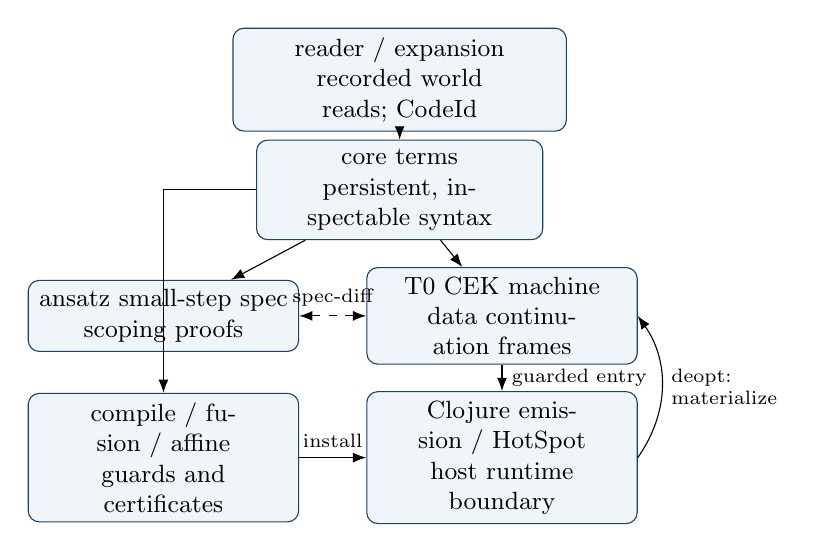
\begin{tikzpicture}[>=Latex,font=\small,box/.style={draw=inkblue,fill=softblue,rounded corners,align=center,minimum height=.85cm}]
\node[box,text width=4cm] (front) at (0,0) {reader / expansion\\recorded world reads; CodeId};
\node[box,text width=3.4cm] (core) at (0,-1.4) {core terms\\persistent, inspectable syntax};
\node[box,text width=3.2cm] (spec) at (-3,-3) {ansatz small-step spec\\scoping proofs};
\node[box,text width=3.2cm] (t0) at (1.3,-3) {T0 CEK machine\\data continuation frames};
\node[box,text width=3.2cm] (compile) at (-3,-4.8) {compile / fusion / affine\\guards and certificates};
\node[box,text width=3.2cm] (host) at (1.3,-4.8) {Clojure emission / HotSpot\\host runtime boundary};
\draw[->] (front)--(core); \draw[->] (core)--(spec); \draw[->] (core)--(t0);
\draw[<->,dashed] (spec)--node[above,font=\scriptsize]{spec-diff}(t0);
\draw[->] (core.west) -| (compile.north);
\draw[->] (compile)--node[above,font=\scriptsize]{install}(host);
\draw[->] (t0)--node[right,font=\scriptsize]{guarded entry}(host);
\draw[->,bend right=35] (host.east) to node[right,font=\scriptsize,align=left]{deopt:\\materialize} (t0.east);
\end{tikzpicture}
\caption{Implemented paths through S11. Dashed spec-diff is testing, not a
refinement proof. The world and authority stores support T0; only the fixed
world and core terms are represented in the current mechanization.}
\label{fig:architecture}
\Description{Core terms connect the reference interpreter, executable formal specification, and compile tier; differential tests compare the first two, and deoptimization reconstructs interpreter frames.}
\end{figure}

\subsection{T0 and the compile tier}
T0 is a CEK-style interpreter whose environments and continuations are data.
This provides a reference execution path, tail calls without growing the host
stack, and inspectable continuations. Host interoperation is deliberately
visible at its effect boundary, although arbitrary internal Java behavior
remains opaque. The local SCI checkout is relevant experience for hosted
Clojure evaluation; Klara's continuation and authority protocols are its own.
Spindel supplies the fork/settlement lineage; Datahike supplies experience with
persistent database roots; Foerster supplies inference workloads. Their larger
protocols are not all implemented by Klara's world adapter.

The compile tier emits Clojure forms and uses the host compiler and HotSpot.
It does not yet generate a standalone native backend or implement the full
self-hosted compiler architecture described in the research notes. S8 adds
world-guarded inlining, conservative partial evaluation, allocation removal
for nonescaping local collections and closures, and direct implementations of
supported tail/abort handlers. Unknown calls must count as possible escape;
representation erasure is licensed only after considering every use.
Unsupported definitions fall back to T0.

S7 memoizes world-guard validity by executable and immutable root identity in
a bounded weak cache. Input-shape and dynamic-handler guards still run at
entry. S9 frame states name source positions by CodeId and path and describe
how live values, constants, closures, recursive closures, and removed vectors
reconstruct T0 state. A deoptimization after an effect resumes at that source
position. It does not replay the entire activation. Branch and staging frames
remain barriers where the reconstruction protocol is unsupported.

S11 adds source loop-header checkpoints. For supported Long and Double loops,
a small abstract interpretation validates invariant argument and backedge
facts, moving checks outside repeated iterations. Arithmetic remains checked;
reassociation, coercion, division, and overflow behavior cannot be changed
merely because a fast numeric representation is available. These passes have
validation and differential tests, not a proved compiler simulation. CodeId
is a SHA-256 digest of canonical expanded syntax, not a proof of semantic
equivalence or an injective mathematical map from all programs.

\subsection{Certificates: what is actually certified}
The fusion path elaborates selected map/filter/reduce pipelines into ansatz
terms over lists of naturals. It uses checked equations
\[
\begin{split}
\kw{foldl}\ f\ b\ (\kw{map}\ g\ xs)
 &=\kw{foldl}\ (\lambda a\,x.f\ a\ (g\ x))\ b\ xs,\\
\kw{foldl}\ f\ b\ (\kw{filter}\ p\ xs)
 &=\kw{foldl}\ (\lambda a\,x.\kw{if}\ (p\ x)\ (f\ a\ x)\ a)\ b\ xs.
\end{split}
\]
Each pipeline has an instantiated equality proof checked at installation.
The optimizer's search is not trusted to assert arbitrary equalities. The
trusted boundary still includes source elaboration into the model, lowering
to host code, correspondence of arithmetic failures, the kernel and imported
initial environment, and the host runtime. A certificate fingerprint records
dependencies; it does not independently re-prove imported declarations.

The entry guard admits realized lists or vectors of nonnegative Longs and
rejects lazy sequences. The host-handler guard prevents bypassing a dynamic
reinterpretation of map, filter, reduce, or arithmetic references. Lowering
uses exact-or-throw arithmetic; overflow deoptimizes to the generic pipeline
from entry, which is permitted only because this fragment is pure. Equality
of overflow behavior is recorded as a trusted, tested obligation. Thus the
claim is a checked equation in a model plus guarded, tested bridges, not a
verified implementation of arbitrary Clojure pipelines. Wandler is the
immediate source of this proof-carrying optimization pattern.

\subsection{Differential specification testing}\label{sec:diff}
The spec-diff harness translates source spec terms to T0 and compares normalized
observations. Its adapter uncurries specialization and let-binds the single
operation clause to avoid evaluating its escapes more often than the spec.
The recorded corpus has 69 cases: 65 agreements and four explicitly asserted
known differences, rather than four silently skipped tests.
\begin{table}[t]
\caption{Known spec/T0 differences in \src{test-spec/klara/spec_diff_test.clj}.}
\small
\begin{tabular}{L{.27\linewidth}L{.29\linewidth}L{.34\linewidth}}
\toprule Case & Spec & T0\\\midrule
Bad perform target & \src{badTarget} & Unhandled lexical effect classification\\
Code value persisted into code & Nested code by substitution & Stage error at lift boundary\\
Closure over generated code variable & Substitution/re-reading changes meaning & Lift refusal\\
Equality on code values & Primitive type error & False\\\bottomrule
\end{tabular}
\end{table}
The observation map collapses closures to a function marker and some opaque
constants to a common token. It can miss extensional differences. The finite
corpus is neither exhaustive nor a proof of the bridge. A systematic numeric
boundary audit is also needed: the spec's mathematical integers and host Long
operations should not be assumed equivalent at overflow.

\section{Recorded Measurements and Their Limits}\label{sec:eval}
We transcribe milestone reports rather than start JVMs on a memory-constrained
machine. The principal comparison is S11's same-session run, OpenJDK 25.0.1,
Clojure 1.12.4, and a 512 MB heap. Each workload uses $n=200$, 100 warmup calls,
and the median of seven batches of 20 calls; compile latency is the median of
five compiles. Times in Table~\ref{tab:bench} are milliseconds per call.
\begin{table}[t]
\caption{S11 recorded microbenchmarks. C/P is compiled/plain Clojure time;
smaller is better. These are workload-specific observations, not general
language speed ratios.}\label{tab:bench}
\small
\begin{tabular}{lrrrrr}
\toprule Workload & T0 & Compiled & Plain & C/P & Compile ms\\\midrule
Numeric loop & .580740 & .006524 & .004918 & 1.327 & 2.911\\
Collections & 1.808210 & .007650 & .020330 & .376 & 12.851\\
Closures & 1.982760 & .015511 & .013793 & 1.125 & 5.337\\
Tail effects & 1.162880 & .011964 & .007014 & 1.706 & 1.981\\\bottomrule
\end{tabular}
\end{table}
Compilation eliminates much of this interpreter's overhead. It does not make
all compiled programs as fast as plain Clojure. The same-session comparison
with the previous implementation reduces the numeric case from 7.901 to
6.524 microseconds and collections from 13.608 to 7.650, while tail effects
increase from 10.794 to 11.964. The report cannot exclude an approximately
11\% regression in that last workload.

A separate, longer-warmed experiment is particularly revealing. After 10,000
warmup calls, with nine batches of 10,000 calls, the $n=200$ numeric loop takes
106 ns and 24 bytes/call in plain Clojure, 99 ns and 24 bytes in the residual
body alone, but 1,536 ns and 4,432 bytes through full compiled entry. At
$n=2000$, times are 847, 784, and 2,027 ns respectively; full-entry allocation
remains 4,432 bytes. These separately warmed measurements are not additive
components to subtract, but show that near-native residual arithmetic can
coexist with roughly $14.5\times$ overhead at the small full-call boundary.

S10's owned-array experiment reports 656, 680, and 680 allocated bytes per call
for zero, 1,000, and one million updates after heavy warmup. Its useful result
is a flat allocation slope between the last two sizes, not zero total
allocation or a general no-allocation theorem. Only a narrow private-array
fragment has this lowering.

These reports provide useful feasibility evidence and falsifiers. They do
not provide independent process repetitions, confidence intervals, a complete
hardware-controlled comparison, large application workloads, or broad tests
of edit-time tail latency and retained memory. Results from different
milestones should not be pooled: workloads, warmup, and implementation changed.
Before submission we propose three evaluation questions: whether repeated
fork/edit/adopt sessions preserve isolation and bounded retention; whether
forced deoptimization at each supported checkpoint preserves effect traces;
and which workload sizes amortize guarded entry and compilation. Benchmark
selection should be fixed before optimization, with unsuccessful cases retained.

\section{Related Work}
\paragraph{Effects and control.}
Algebraic handlers separate effect requests from interpretations~\cite{plotkin2009}.
Klara uses this separation to expose alternative futures, but adds a store
that can reject duplication of authority. Effekt's lexical capabilities make
handler identity a scoping question and support static effect reasoning
\cite{effekt2020}. Koka's generalized evidence passing attacks handler dispatch
and control overhead~\cite{koka2021}. Klara instead starts with dynamic checks
and attempts to discharge selected obligations by local facts and guards;
it does not inherit either language's type safety. OCaml's retrofit emphasizes
one-shot continuations and integration with an existing runtime~\cite{ocaml2021}.
Klara's persistent data continuations support repeated resumption within T0,
but the host boundary and authority footprint limit when it is legal.

\paragraph{Staging.}
MetaML supplies the code/escape tradition and static cross-stage guarantees
\cite{metaml2000}; BER MetaOCaml supplies dynamic scope-extrusion checking
\cite{ber2014}. Klara adopts the latter problem boundary without a typed
object language. LMS separates binding times through a library and generated
IR~\cite{lms2010}; Amin and Rompf demonstrate how stage-polymorphic evaluators
can collapse towers of interpretation~\cite{amin2018}. Klara's staged
interpreter example explores that direction. Its value-level \src{specialize}
rule alone is only partial application, not a claim that a compiler appears
without an optimizer, backend, and correctness argument.

\paragraph{Language extension and hosted interaction.}
Racket's languages-as-libraries approach exposes expansion and static semantics
as programmable interfaces~\cite{racket2011}. Klara aims to make such extensions
world-resident and dependent on recorded reads, but full syntax objects and
the broader language-extension lattice remain design work. Clojure supplies
persistent data, hosted execution, and the interactive idiom~\cite{clojure2020}.
Klara moves definition lookup into explicit immutable worlds; linked Clojure
state is still shared host state. Unison's content-addressed definitions
provide a useful comparison~\cite{unison}: CodeId identifies Klara's expanded
syntax, while mutable names, captured bases, and guarded executables remain
separate concerns. Neither hashes nor alpha-equivalence implement the
unforgeable nominal seals proposed in RFC 0007.

\paragraph{Optimization and verification.}
Truffle/Graal demonstrates the combination of interpreter specialization and
an optimizing runtime~\cite{truffle2013}. Klara's world immutability permits
validity memoization by root; source-level frame states support returning to
T0 without host stack surgery. The proof obligation is still reconstruction
of the exact source state after effects. CakeML exemplifies a substantially
stronger end-to-end verification boundary~\cite{cakeml2014}. WebAssembly's
mechanization illustrates the value of executable specification and validation
against implementations~\cite{watt2018}. Klara is closer to a small proved
reference model plus differential testing and selected certificates than to
an end-to-end verified compiler.

\paragraph{Resources, probability, and joins.}
Fractional permissions~\cite{boyland2003} and Iris resource algebras
\cite{iris2018} supply the vocabulary for stating ownership compatibility;
they do not automatically justify Klara's particular settlement protocol.
Probabilistic semantics must account for scores and normalization, rather than
merely enumerate weighted branches~\cite{staton2016}. The adjacent
$\lambda_\vee$ project makes evidence identity, split, and join explicit.
Its local Lean development includes preservation and no-double-counting
results for its own footprint calculus; its Redex model uses tests to find
bad copying rules. The related unpublished draft \emph{Every Join Has a Base:
Merging What Forked Computations Learned} separates base, identification,
weights, and residual policy~\cite{joinsdraft}. Those distinctions motivate
Klara's authority design, but none of those proofs currently transfers to
Klara's CEK machine. A general join of alternative computations is also
stronger than the implemented at-most-one-branch adoption operation.

\section{Limitations and Next Research Steps}
The most important missing result concerns the paper's central idea:
conservation and nonduplication of authority are implemented but outside the
mechanized core. Extending configurations with $\Sigma$, branch contexts,
loans, generations, and settlement outcomes would let the paper state what
``forkable'' means beyond persistent snapshots. A first tractable theorem is
stale-token rejection and conservation for exclusive resources, evidence,
and read loans under sequential forks; recovery and concurrent settlement
should be separate extensions.

The staging proofs preserve de Bruijn scoping, but do not yet prove generated
name freshness, capability uniqueness, or binder-general run/quote laws.
The front end, executable spec bridge, T0, and emitted host code remain
unverified connections. Four acknowledged spec differences and numeric
representation gaps need either reconciliation or an explicit refinement
relation. The denotational proposal is only a finite discrete algebra; full
higher-order adequacy and a model of intensional code remain open.

The host is the largest practical boundary. Raw mutable objects, unrecorded
macro reads, retrying publications that can repeat definition-time effects,
and unclassified irreversible calls can escape the intended world account.
S10's static checker covers local islands, not a whole-program affine type
system. Let-insertion shares mutable generation loci across repeated resumptions.
The design's JS, Wasm, native, storage-tier, and self-hosting paths are research
plans, not implemented portability claims.

For the next paper iteration, we suggest keeping the narrative centered on
forking and authority, using staging and deoptimization as the test of whether
that account survives optimization. The decision is substantive: either add
a small authority preservation theorem and use the compiler as supporting
evidence, or make the paper an explicitly empirical language-design study
with much stronger workloads. The present manuscript supports that choice
without hiding which parts are already checked.

\section*{Data Availability}
This internal artifact contains the LaTeX source, bibliography, build
instructions, venue survey, citation/source ledger, and discussion issues in
\src{paper/}. Examples and measurements are transcribed from the repository's
executable guides and S1--S11 reports at the snapshot stated on page 1.
No new performance measurements or proof runs were performed. A public,
anonymized archival artifact and stable repository URL remain to be prepared
for submission; local private Zotero data and personal notes are excluded.

\section*{Use of Generative AI}
This internal draft was prepared with an AI coding assistant for repository
inspection, literature and venue searches, drafting, and LaTeX production.
Christian Weilbach has not yet reviewed or endorsed its new definitions,
proof sketches, or interpretations. The named authorship is a discussion-draft
placeholder, not a representation that the manuscript has been approved for
submission. The bibliography was checked against primary sources; the remaining
research obligations are explicitly labeled.

\bibliographystyle{ACM-Reference-Format}
\bibliography{references}
\end{document}
